\documentclass[12pt,a4paper]{article}
\usepackage[utf8]{inputenc}
\usepackage[english]{babel}
\usepackage{amsmath}
\usepackage{amsfonts}
\usepackage{amssymb}
\usepackage{latexsym}
\usepackage{makeidx}
\usepackage{graphicx}
\usepackage{graphics}
\usepackage{lmodern}
\usepackage{hyperref}
\usepackage{subcaption}
\usepackage{pgfplots}
\usepackage{dsfont}
\usepackage{multicol}
\usepackage{xcolor}
\usepackage{booktabs}
\usepackage{float}
\usepackage{subcaption}
\pgfplotsset{width=10cm,compat=1.9}
\usepgfplotslibrary{external}
\usepackage{fancybox}


\setlength{\parindent}{0px}
\usepackage[left=2cm,right=2cm,top=4cm,bottom=2cm]{geometry}

\author{Daniel Vázquez Lago}
\title{Apuntes Métodos Matemáticos VI}

\newcommand{\parentesis}[1]{\left( #1  \right)}
\newcommand{\parciales}[2]{\frac{\partial #1}{\partial #2}}
\newcommand{\pparciales}[2]{\parentesis{\parciales{#1}{#2}}}
\newcommand{\ccorchetes}[1]{\left[ #1  \right]}
\newcommand{\D}{\mathrm{d}}
\newcommand{\sech}{\mathrm{sech} \ }
\newcommand{\csch}{\mathrm{csch} \ }

\begin{document}

\maketitle

\newpage

\tableofcontents\documentclass[12pt,a4paper]{article}
\usepackage[utf8]{inputenc}
\usepackage[english]{babel}
\usepackage{amsmath}
\usepackage{amsfonts}
\usepackage{amssymb}
\usepackage{latexsym}
\usepackage{makeidx}
\usepackage{graphicx}
\usepackage{graphics}
\usepackage{lmodern}
\usepackage{hyperref}
\usepackage{subcaption}
\usepackage{pgfplots}
\usepackage{dsfont}
\usepackage{multicol}
\usepackage{xcolor}
\usepackage{booktabs}
\usepackage{float}
\usepackage{subcaption}
\pgfplotsset{width=10cm,compat=1.9}
\usepgfplotslibrary{external}
\usepackage{fancybox}


\setlength{\parindent}{0px}
\usepackage[left=2cm,right=2cm,top=4cm,bottom=2cm]{geometry}

\author{Daniel Vázquez Lago}
\title{Apuntes Métodos Matemáticos VI}

\newcommand{\parentesis}[1]{\left( #1  \right)}
\newcommand{\parciales}[2]{\frac{\partial #1}{\partial #2}}
\newcommand{\pparciales}[2]{\parentesis{\parciales{#1}{#2}}}
\newcommand{\ccorchetes}[1]{\left[ #1  \right]}
\newcommand{\D}{\mathrm{d}}
\newcommand{\sech}{\mathrm{sech} \ }
\newcommand{\csch}{\mathrm{csch} \ }

\begin{document}

\maketitle

\newpage

\tableofcontents

\newpage


\newpage


\section{Plano complejo}

\section{Funciones de variable compleja}

\subsection*{Variables y funciones}

Llamamos \textit{variable compleja} a cualquier elemento (simbolizado por $z$, $w \ldots$) que representa cualquier elemento de un conjunto de números complejos. \\

Si a cada valor que puede tomar la variable compleja $z$ le corresponde (asignamos al valor $z$) uno o más valores de una variable $w$, decimos que $w$ es una \textit{función} de $z$ y escribimos $w=f(z)$. La variable $z$ es denominada la \textit{variable independiente} y la variable $w$ la \textit{variable dependiente}.

\subsection*{Funciones univocas y mutivocas}

Si a cada valor de $z$ corresponde sólo un valor de $w$, decimos que $w$ es una \textit{función unívoca} de $z$ o que $f(z)$ es unívoca. Si más de de un valor de $w$ corresponde a cada valor de $z$, decimos que $w$ es una \textit{función multívoca} de $z$. \\

Una función multievaluada puede considerarse como una colección de funciones unívocas, donde cada miembro es llamado \textit{rama} de la función.  \\


\shadowbox{\textbf{Ejemplo 2.1 y 2.2}}

\hrulefill
\begin{itemize}

\item \textbf{Ejemplo 2.1:} si $w = z^2$, entonces para cada valor de z existe un solo valor de $w$. Por lo tanto es una función univoca de z.

\item \textbf{Ejemplo 2.2:} si $w = z^{1/2}$, entonces para cada valor de $z$ existen dos valores de $w$. Por lo tanto es una función multívoca (bivaluada) de $z$. 

\end{itemize}
\hrulefill \\

\subsection*{Trasformaciones}

Si $w = u +iv$ y $z = x+iy$ podemos considerar la función $w=f(z)$ como $u+iv = f(x+iy)$. Entonces como sabemos podemos escribir $x+iy $ como $(x,y)$ y entoncces la función $f$ es una función análoga a $\mathbb{R}^2 \rightarrow \mathbb{R}^2$. Es equivalente a:

\begin{equation}
u = u(x,y) \ \ v=v(x,y)
\end{equation}

Entonces a cada punto $(x,y)$ en el plano $z$, tal como $P$, le corresponde el punto $(u,v)$ en el plano $w$, digamos $P'$. Entonces decimos que en el punto $P$ se \textit{aplica o transforma} en el punto $P'$, llamado \textit{imagen} de $P$.

\subsection*{Funciones elementales}


\begin{enumerate}

\item \textbf{Funciones polinomiales} son las definidas por

\begin{equation}
w = a_n z^n + \cdots + a_2 z^2 + a_1 z + a_0
\end{equation}

donde $a_n \neq 0, \ldots, a_2, a_1, a_0$ son constantes complejas.

\item \textbf{Funciones alegraicas racionales} son las definidas por 

\begin{equation}
w  = \dfrac{P(z)}{Q(z)}
\end{equation}

donde $P(z)$ y $Q(z)$ son polinomios.

\item \textbf{Funciones exponenciales} son las definidas por 

\begin{equation}
w = e^z = e^x (\cos y + i \sin y)
\end{equation}

Si $a$ es real y positivo definimos:

\begin{equation}
a^z = e^{z \ln a}
\end{equation}

\item \textbf{Funciones trigonométricas.} Definimos las funciones trigonométricas en términos de las funciones exponenciales:

\begin{equation}
\begin{array}{cclccclc}

\sin z & = & \dfrac{e^{iz}-e^{-iz}}{2i} & \ \ \ \ \ \ \ \ & \cos z & = & \dfrac{e^{iz} + e^{-iz}}{2} \\ \\

\sec z & = & \dfrac{1}{\cos z} = \dfrac{2}{e^{iz}+e^{-iz}} & \ & \csc z& = & \dfrac{1}{\sin z} = \dfrac{2i}{e^{iz}-e^{-iz}} \\ \\

\tan z & = & \dfrac{\sin z}{\cos z} = \dfrac{e^{iz}-e^{-iz} }{i (e^{iz}+e^{-iz})} & & \cot z & = & \dfrac{\cos z}{\sin z} = \dfrac{i(e^{iz}+e^{-iz})}{(e^{iz}-e^{-iz})} 

\end{array}
\end{equation}

La mayoría de las propiedades de las funciones trigonométricas reales son válidas para las funciones complejas, como

\begin{equation}
\sin^2 z + \cos^2 z = 1; \ \ \sin(-z) = - \sin(z); \ \ \cos (-z) = \cos (z) \ldots
\end{equation}

además de las funciones angulo doble, ángulo mitad... De hecho estas se pueden deducir directamente de las expresiones complejas.


\item  \textbf{Funciones hiperbólicas} son las definidas como

\newpage

\begin{equation}
\begin{array}{cclccclc}

\sinh z & = & \dfrac{e^{z}-e^{-z}}{2} & \ \ \ \ \ \ \ \ & \cosh z & = & \dfrac{e^{z} + e^{-z}}{2} \\ \\

\sech z & = & \dfrac{1}{\cosh z} = \dfrac{2}{e^{z}+e^{-z}} & \ & \csch z& = & \dfrac{1}{\sinh z} = \dfrac{2i}{e^{z}-e^{-z}} \\ \\

\tanh z & = & \dfrac{\sinh z}{\cosh z} = \dfrac{e^{z}-e^{-z} }{ (e^{z}+e^{-z})} & & \coth z & = & \dfrac{\cosh z}{\sinh z} = \dfrac{(e^{z}+e^{-z})}{(e^{z}-e^{-z})} 

\end{array}
\end{equation}

Siendo las siguientes propiedades válidas

\begin{equation}
\cosh^2 z - \sinh^2 z = 1; \ \ \sinh (-z) = - \sinh (z); \ \ \cosh (-z) = \cosh (z) \ldots
\end{equation}


Lo mas destacable de estas funciones es que están relacionadas con las funciones trigonométricas, de la siguiente forma:

\begin{equation}
\sin iz = i \sinh z; \ \ \ \ \cos iz = \cosh z
\end{equation}

\item \textbf{Funciones logarítmicas.} Es la función inversa de la función exponencial, y es multivaluada ya que si $z = r e^{i \theta} = r e^{\theta + 2k \pi}$ tenemos que:

\begin{equation}
\ln z = \ln r + i (\theta + 2k \pi) \ \ \ k = 0, \pm 1, \pm2, \ldots
\end{equation}

En este caso la \textit{rama principal} de la función logaritmo se define para $k=0$, es decir:

\begin{equation}
\ln z = ln r + \i \theta
\end{equation}


\item \textbf{Funciones trigonométricas inversas.} Si $z = \sin w$, entonces $w = \sin^{-1}$ se llama \textit{seno inverso de z} o \textit{arcoseno de z}. Son todas ellas funciones multivaluadas, y se expresan en términos de logaritmos naturales:

\begin{equation}
\begin{array}{cclccclc}

\sin^{-1} z & = & \dfrac{1}{i} \ln (i z + \sqrt{1-z^2}) & \ \ \ \ \ \ \ \ & \cos^{-1} z & = & \dfrac{1}{i} \ln (i z + \sqrt{z^2-1}) \\ \\

\sec^{-1} z & = & \dfrac{1}{i} \ln \parentesis{\dfrac{1 + \sqrt{1-z^2}}{z}} & \ \ & \csc^{-1} z & = & \dfrac{1}{i} \ln  \parentesis{\dfrac{i + \sqrt{z^2-1}}{z}} \\ \\

\tan^{-1} z & = & \dfrac{1}{2i} \ln  \parentesis{\dfrac{1 + i z}{1-iz}} & & \cot^{-1} z & = & \dfrac{1}{2i} \ln  \parentesis{\dfrac{z + i }{z-i}}

\end{array}
\end{equation}

\item \textbf{Funciones hiperbólicas inversas.} Si $z = \sinh w$ entonces $w = \sinh^{-1} z$, se llama \textit{seno hiperbólico inverso de z}. Son funciones multivaluadas, que se expresan en función del logaritmo natural:


\begin{equation}
\begin{array}{cclccclc}

\sinh^{-1} z & = & \ln (z + \sqrt{z^2+1}) & \ \ \ \ \ \ \ \ & \cosh^{-1} z & = & \ln (z + \sqrt{z^2-1}) \\ \\

\sech^{-1} z & = &  \ln \parentesis{\dfrac{1+\sqrt{1-z^2}}{z}} & \ & \csch^{-1} z& = & \ln \parentesis{\dfrac{1+\sqrt{z^2+1}}{z}} \\ \\

\tanh^{-1} z & = & \dfrac{1}{2} \ln  \parentesis{\dfrac{1 + z}{1-z}} & & \coth^{-1} z & = &  \dfrac{1}{2} \ln  \parentesis{\dfrac{z + 1 }{z-1}}

\end{array}
\end{equation}
\end{enumerate}
\subsection*{Puntos de ramificacion y ramas}

Supongamos que nos han dado la función  $w = \sqrt{z}$. Supongamos que además dejamos que $z$ de una vuelta entera alrededor del origen empezando en A. Tenemos entonces que $z=re^{i\theta_1}$ entonces $w = \sqrt{r} e^{i \theta-1 /2}$. Después de una vuelta completa $\theta = \theta_1 + 2\pi$; tenemos que $w = \sqrt{r} e^{i (\theta_1 +2 \pi)/2} = - \sqrt{r} e^{i \theta_1 /2}$. Entonces no hemos obtenido el mismo valor de $w$ que al comienzo. Sin embargo si damos dos vueltas $\theta = \theta_1 + 4 \pi$, obtenemos el mismo valor que al principio.  \\

Podemos describir lo anterior diciendo que si $0 \leq \theta < 2 \pi$ estamos en una rama de la función multivaluada $z^{1/2}$, mientras que si $ 2 \pi \leq \theta < 4 \pi $ estamos en otra rama. \\

Está claro que cada rama es unívoca. Con el fin de mantener la función unívoca (para que sea diferenciable y continua), creamos una barrera artificial $OB$, donde $B \rightarrow \infty$, que podemos ver en la figura, la cual acordamos no cruzar. No es que no se pueda cruzar, ni que sea imposible, solo es un artificio mental para que la función sea unívoca. Esta barrera, representada por una línea gruesa en la figura, se llama \textit{rama}, y el punto $O$ \textit{punto de ramificación}. Esto es porque si damos la vuelta alrededor de cualquier otro punto $z$ no se conduce a valores diferentes. 


\begin{figure}[h!] \centering
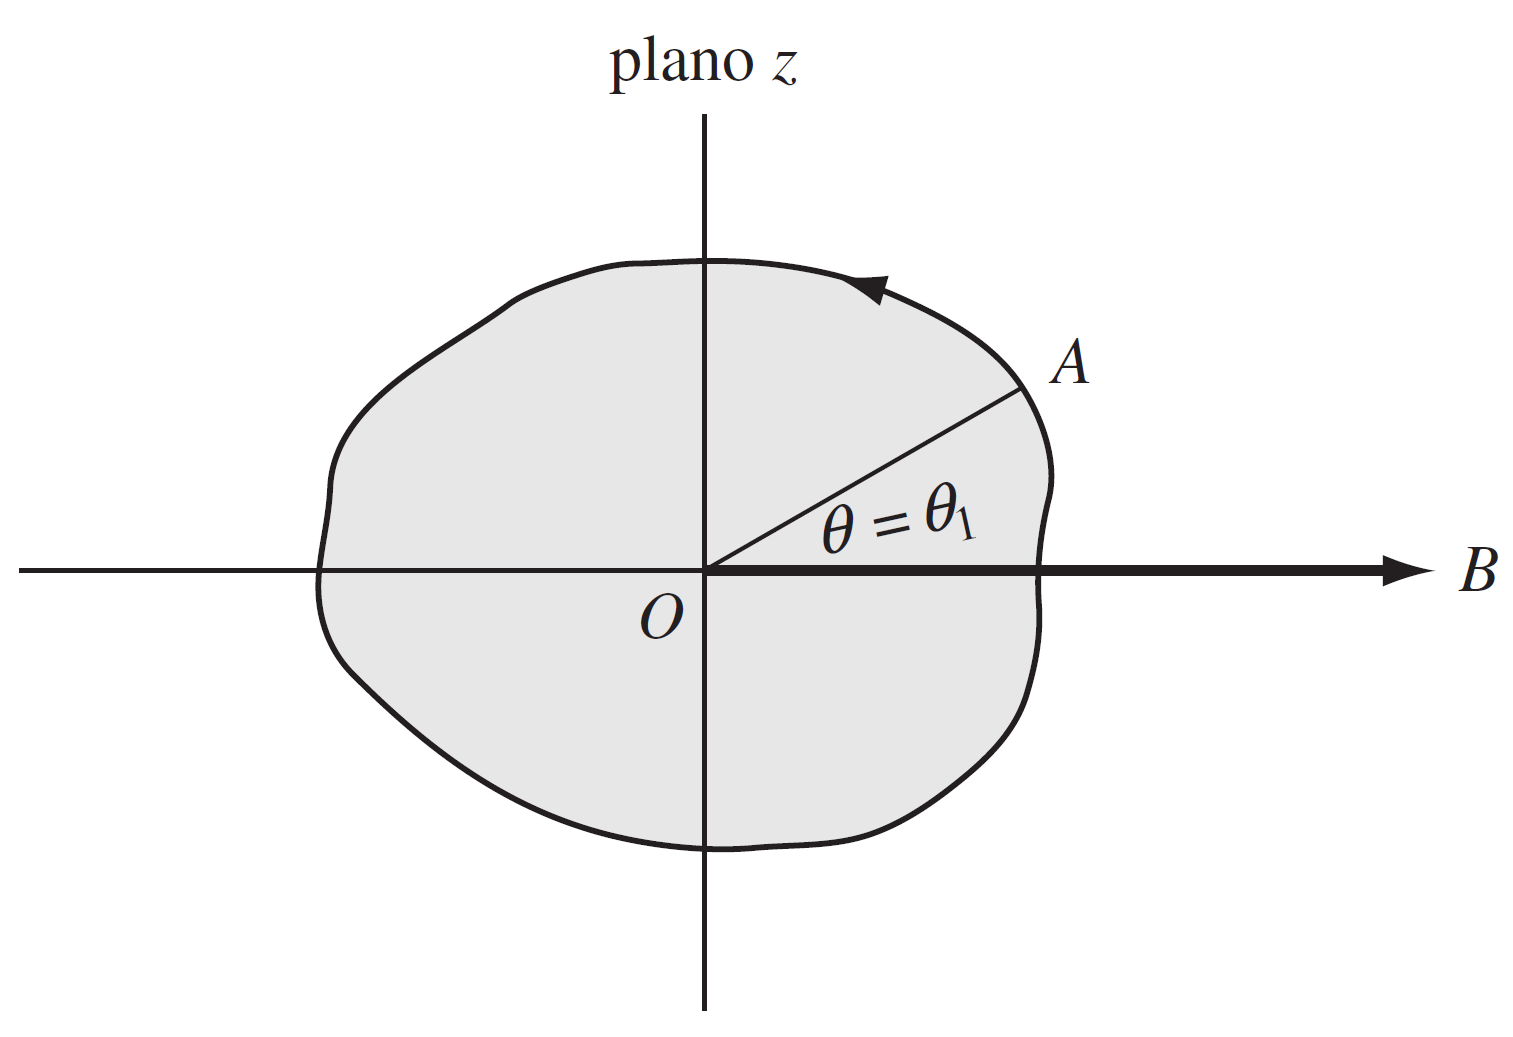
\includegraphics[scale=0.3]{ramificaciones.png}
\caption{Ejemplo de ramificación}
\end{figure}



\subsection*{Superficies de Riemann} 

Existe una manera análoga de lograr lo mismo que con la línea de ramificación. Para esto debemos imaginarnos el plano $z$ como dos capas superpuestas, ambas cortadas por la recta $OB$, y que el borde inferior de la capa inferior se une con el borde superior de la capa superior, de tal modo que si se continúa dando vueltas se va de la capa superior a la capa inferior y así recurrentemente. \\

El caso de dos capas corresponden a la función $z^{1/2}$, pero evidentemente puede haber mas superficies de Riemann con mas capas. El conjunto de todas las capas hace la \textit{superficie de Riemann}. Por ejemplo para la función $w = \ln z$ existen infinitas capas.

\subsection*{Límites}

Los límites se definen de manera análoga a como se hace en el caso real, o de $\mathbb{R}^n$. Decimos que A es el límite de $f(z)$ tendiendo a $z_0$ como:

\begin{equation}
\lim_{z \rightarrow z_0} f(z)  = A  \ \ \mathrm{si} \ \forall \ \epsilon > 0, \ \epsilon \in \mathbb{R} \  \exists \ \delta \ / \ A - f(z) < \epsilon   \ \forall \ z \ \mathrm{tal \ que} \ z-z_0 < \delta
 \end{equation}

Cuando estamos en funciones multivaluadas en general el límite depende de en que rama nos encontremos. Además mucho de los teoremas sobre límites para funciones reales son válidos para funciones complejas, tales como:

\begin{equation}
\lim_{z \rightarrow z_0} (f(z)+g(z)) = \lim_{z \rightarrow z_0} f(z) + \lim_{z \rightarrow z_0} g(z)
\end{equation}

\begin{equation}
\lim_{z \rightarrow z_0} (f(z) g(z)) = \ccorchetes{\lim_{z \rightarrow z_0} f(z)} \cdot \ccorchetes{\lim_{z \rightarrow z_0} g(z) }
\end{equation}

\begin{equation}
\lim_{z \rightarrow z_0}  \dfrac{f(z)}{g(z)} = \dfrac{\lim_{z \rightarrow z_0}  f(z)}{\lim_{z \rightarrow z_0} g(z)} \ \mathrm{si} \ \lim_{z \rightarrow z_0} g(z) \neq 0
\end{equation}



\shadowbox{\textbf{Ejemplo 2.3}}

\hrulefill

Vamos a demostrar que el limite  $\lim_{z \rightarrow 0} \bar{z}/z$ no existe. \\

Si existiera el límite está claro que da igual el camino escogido para llegar al punto 0, debe dar igual que dirección cojamos al aproximarnos. Entonces estudiaremos la mas básica. Si $z=x+iy$, una condición para que exista límite: 

\begin{equation}
\lim_{x \rightarrow 0} \lim_{y \rightarrow 0} f(z) = \lim_{y \rightarrow 0} \lim_{x \rightarrow 0} f(z)
\end{equation}

Si ahora comprobamos eso para la función $\frac{x-iy}{x+iy}=f(z)$:

$$ \lim_{x \rightarrow 0} \lim_{y \rightarrow 0} \frac{x-iy}{x+iy} = \lim_{x \rightarrow 0} \dfrac{x}{x} = 1 $$

$$ \lim_{y \rightarrow 0} \lim_{x \rightarrow 0} \frac{x-iy}{x+iy} =  \lim_{y \rightarrow 0} \frac{-iy}{iy} = -1 $$

\hrulefill \\


\end{document}

